%%%%%%%%%%%%%%%%%%%%%%%%%%%%%%%%%%%%%%%%%
% Beamer Presentation
% LaTeX Template
% Version 2.0 (March 8, 2022)
%
% This template originates from:
% https://www.LaTeXTemplates.com
%
% Author:
% Vel (vel@latextemplates.com)
%
% License:
% CC BY-NC-SA 4.0 (https://creativecommons.org/licenses/by-nc-sa/4.0/)
%
%%%%%%%%%%%%%%%%%%%%%%%%%%%%%%%%%%%%%%%%%

%----------------------------------------------------------------------------------------
%       PACKAGES AND OTHER DOCUMENT CONFIGURATIONS
%----------------------------------------------------------------------------------------

\documentclass[
        11pt, % Set the default font size, options include: 8pt, 9pt, 10pt, 11pt, 12pt, 14pt, 17pt, 20pt
        %t, % Uncomment to vertically align all slide content to the top of the slide, rather than the default centered
        %aspectratio=169, % Uncomment to set the aspect ratio to a 16:9 ratio which matches the aspect ratio of 1080p and 4K screens and projectors
]{beamer}

\graphicspath{{Images/}{./}} % Specifies where to look for included images (trailing slash required)

\usepackage{booktabs} % Allows the use of \toprule, \midrule and \bottomrule for better rules in tables

%----------------------------------------------------------------------------------------
%       SELECT LAYOUT THEME
%----------------------------------------------------------------------------------------

% Beamer comes with a number of default layout themes which change the colors and layouts of slides. Below is a list of all themes available, uncomment each in turn to see what they look like.

%\usetheme{default}
%\usetheme{AnnArbor}
%\usetheme{Antibes}
%\usetheme{Bergen}
%\usetheme{Berkeley}
%\usetheme{Berlin}
%\usetheme{Boadilla}
%\usetheme{CambridgeUS}
%\usetheme{Copenhagen}
%\usetheme{Darmstadt}
%\usetheme{Dresden}
%\usetheme{Frankfurt}
%\usetheme{Goettingen}
%\usetheme{Hannover}
%\usetheme{Ilmenau}
%\usetheme{JuanLesPins}
%\usetheme{Luebeck}
\usetheme{Madrid}
%\usetheme{Malmoe}
%\usetheme{Marburg}
%\usetheme{Montpellier}
%\usetheme{PaloAlto}
%\usetheme{Pittsburgh}
%\usetheme{Rochester}
%\usetheme{Singapore}
%\usetheme{Szeged}
%\usetheme{Warsaw}

%----------------------------------------------------------------------------------------
%       SELECT COLOR THEME
%----------------------------------------------------------------------------------------

% Beamer comes with a number of color themes that can be applied to any layout theme to change its colors. Uncomment each of these in turn to see how they change the colors of your selected layout theme.

%\usecolortheme{albatross}
%\usecolortheme{beaver}
%\usecolortheme{beetle}
%\usecolortheme{crane}
%\usecolortheme{dolphin}
%\usecolortheme{dove}
%\usecolortheme{fly}
%\usecolortheme{lily}
%\usecolortheme{monarca}
%\usecolortheme{seagull}
%\usecolortheme{seahorse}
%\usecolortheme{spruce}
%\usecolortheme{whale}
%\usecolortheme{wolverine}

%----------------------------------------------------------------------------------------
%       SELECT FONT THEME & FONTS
%----------------------------------------------------------------------------------------

% Beamer comes with several font themes to easily change the fonts used in various parts of the presentation. Review the comments beside each one to decide if you would like to use it. Note that additional options can be specified for several of these font themes, consult the beamer documentation for more information.

\usefonttheme{default} % Typeset using the default sans serif font
%\usefonttheme{serif} % Typeset using the default serif font (make sure a sans font isn't being set as the default font if you use this option!)
%\usefonttheme{structurebold} % Typeset important structure text (titles, headlines, footlines, sidebar, etc) in bold
%\usefonttheme{structureitalicserif} % Typeset important structure text (titles, headlines, footlines, sidebar, etc) in italic serif
%\usefonttheme{structuresmallcapsserif} % Typeset important structure text (titles, headlines, footlines, sidebar, etc) in small caps serif

%------------------------------------------------

%\usepackage{mathptmx} % Use the Times font for serif text
\usepackage{palatino} % Use the Palatino font for serif text

%\usepackage{helvet} % Use the Helvetica font for sans serif text
\usepackage[default]{opensans} % Use the Open Sans font for sans serif text
%\usepackage[default]{FiraSans} % Use the Fira Sans font for sans serif text
%\usepackage[default]{lato} % Use the Lato font for sans serif text

%----------------------------------------------------------------------------------------
%       SELECT INNER THEME
%----------------------------------------------------------------------------------------

% Inner themes change the styling of internal slide elements, for example: bullet points, blocks, bibliography entries, title pages, theorems, etc. Uncomment each theme in turn to see what changes it makes to your presentation.

%\useinnertheme{default}
\useinnertheme{circles}
%\useinnertheme{rectangles}
%\useinnertheme{rounded}
%\useinnertheme{inmargin}

%----------------------------------------------------------------------------------------
%       SELECT OUTER THEME
%----------------------------------------------------------------------------------------

% Outer themes change the overall layout of slides, such as: header and footer lines, sidebars and slide titles. Uncomment each theme in turn to see what changes it makes to your presentation.

%\useoutertheme{default}
%\useoutertheme{infolines}
%\useoutertheme{miniframes}
%\useoutertheme{smoothbars}
%\useoutertheme{sidebar}
%\useoutertheme{split}
%\useoutertheme{shadow}
%\useoutertheme{tree}
%\useoutertheme{smoothtree}

%\setbeamertemplate{footline} % Uncomment this line to remove the footer line in all slides
%\setbeamertemplate{footline}[page number] % Uncomment this line to replace the footer line in all slides with a simple slide count

%\setbeamertemplate{navigation symbols}{} % Uncomment this line to remove the navigation symbols from the bottom of all slides

%----------------------------------------------------------------------------------------
%       PRESENTATION INFORMATION
%----------------------------------------------------------------------------------------

\title[FMatC]{Formal Methods above the Code} % The short title in the optional parameter appears at the bottom of every slide, the full title in the main parameter is only on the title page

\subtitle{specifying a non-computer} % Presentation subtitle, remove this command if a subtitle isn't required

\author[]{Martin Ames Harrison} % Presenter name(s), the optional parameter can contain a shortened version to appear on the bottom of every slide, while the main parameter will appear on the title slide

\institute[RTX BBN]{} % Your institution, the optional parameter can be used for the institution shorthand and will appear on the bottom of every slide after author names, while the required parameter is used on the title slide and can include your email address or additional information on separate lines

\date[\today]{RTX BBN Interview \\ \today} % Presentation date or conference/meeting name, the optional parameter can contain a shortened version to appear on the bottom of every slide, while the required parameter value is output to the title slide

%----------------------------------------------------------------------------------------

\begin{document}

%----------------------------------------------------------------------------------------
%       TITLE SLIDE
%----------------------------------------------------------------------------------------

\begin{frame}
        \titlepage % Output the title slide, automatically created using the text entered in the PRESENTATION INFORMATION block above
\end{frame}

%----------------------------------------------------------------------------------------
%       TABLE OF CONTENTS SLIDE
%----------------------------------------------------------------------------------------

% The table of contents outputs the sections and subsections that appear in your presentation, specified with the standard \section and \subsection commands. You may either display all sections and subsections on one slide with \tableofcontents, or display each section at a time on subsequent slides with \tableofcontents[pausesections]. The latter is useful if you want to step through each section and mention what you will discuss.

\begin{frame}
        \frametitle{Some Background} % Slide title, remove this command for no title
        \begin{figure}
                
\includegraphics[width=\linewidth]{backgroundPic.png}
        \end{figure}
\end{frame}

\begin{frame}
    \frametitle{About DeepSpec} 
    \begin{itemize}
        \item NSF \emph{Expedition in Computing} focused on "the specification and verification of full functional correctness of software and hardware"
        \item vision: build systems with end-to-end formal verification of specs
        \item tools include Coq/Gallina among many others (next slide)
    \end{itemize}
\end{frame}

\begin{frame}
    \frametitle{DeepSpec in a Picture}
        \begin{figure}
            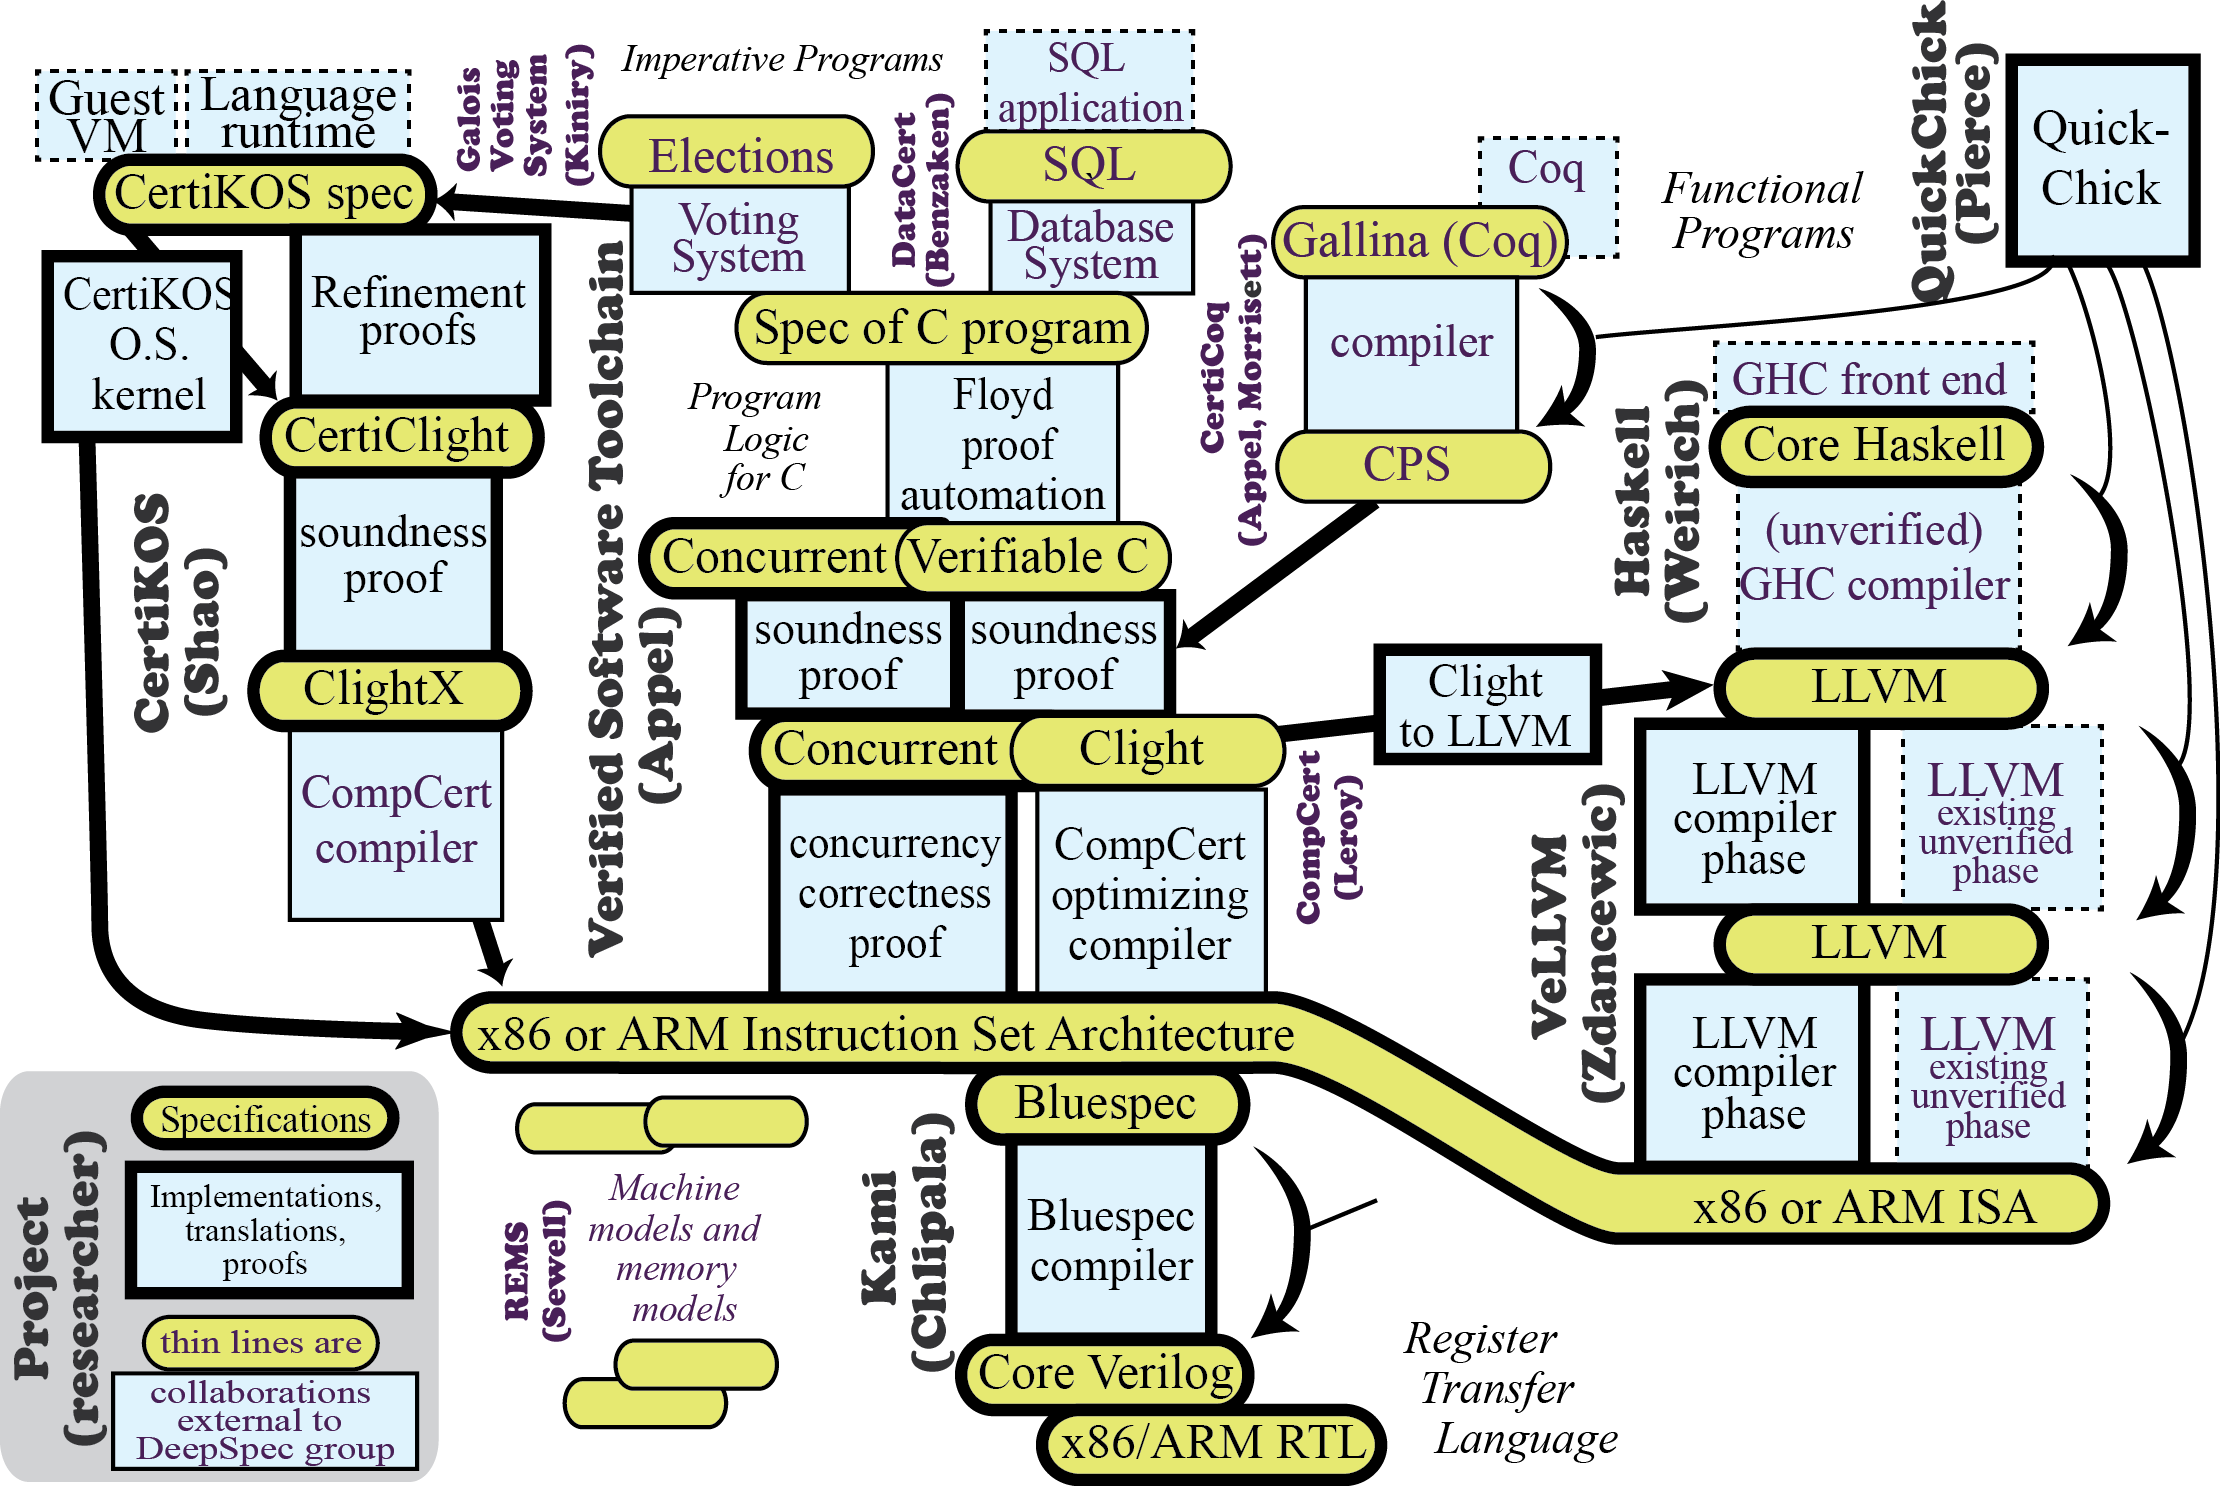
\includegraphics[width=.9\linewidth]{SpecBox.png}
        \end{figure}
\end{frame}

\begin{frame}
    \frametitle{Verified Missile Toolchain?}
        \begin{itemize}
            \item Can we mimic this in MDA's software IV\&V operation?
            \item IV\&V = Independent Verification \& Validation
            \begin{itemize}
                \item contractor delivers code to customer
                \item independent entity evaluates code, reports findings
                \item repeat till final delivery
            \end{itemize}
            \item {\bf idea}: let's use Coq to develop in parallel, producing corrected and verified versions of contractors' code drops
            \item {\bf plan}: hire a dozen STEM types and put them to work studying \emph{Software Foundations} in IV\&V lab
            \item {\bf result}: skepticism, chairs thrown and a {\bf new task}!
        \end{itemize}
\end{frame}

\begin{frame}
    \frametitle{A Different Approach}
    \begin{columns}[c]
        \begin{column}{.6\textwidth}
        \begin{itemize}
            \item begin formal methods practice at the outset of a project, at the \emph{system design level}
            \item NASA used PVS for collision-avoidance algorithms
            \item Lamport's TLA+ used in RTOS design
            \item TLA+ used also by Elasticsearch in developing their data replication algorithm
        \end{itemize}
        \end{column}
        \begin{column}{.4\textwidth}
        \begin{figure}
            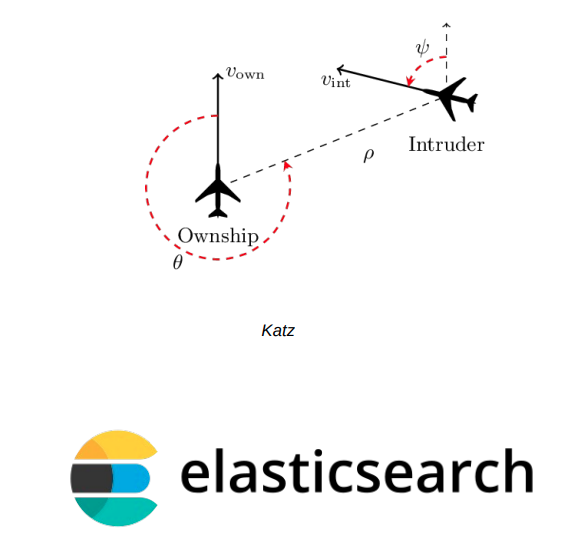
\includegraphics[width=.9\linewidth]{demoSystems.png}
        \end{figure}
        \end{column}
    \end{columns}
\end{frame}

\begin{frame}
    \frametitle{On TLA+ and Model Checking}
    \begin{itemize}
        \item describes system as a finite state machine
        \item allowed transitions ({\bf actions}) are specified together with initial state
        \item has {\bf constants}, knobs to adjust model scale
        \item the TLC model checker searches breadth-first the reachable states of the system, checking {\bf state} predicates and {\bf behavior} properties
        \item feature of interest: TLA+ supports {\bf refinement} or {\bf implementation}; checking or proving that one spec is a higher resolution picture of another
    \end{itemize}
\end{frame}

\begin{frame}
    \frametitle{On Refinement}
    What is refinement,exactly? We need some terms:\

    \begin{itemize}
        \item an {\bf action} is a predicate on (state, next state) pairs
        \item a {\bf behavior} is a sequence of states
        \item a spec is a set of valid behaviors
        \item spec B {\bf refines} spec A if there is a map from B's state into A's state such that all valid behaviors of B map to valid behaviors of A
    \end{itemize}
    Let's look at an example!
\end{frame}

\begin{frame}
    \frametitle{Polymerase Chain Reaction}
    \begin{columns}[c]
        \begin{column}{.4\textwidth}
        \begin{itemize}
            \item invented by Kary Mullis in 1983; won Nobel
            \item amplifies desired snippet of DNA (called \emph{amplion})
            \item requires \emph{thermal cycling}, \emph{primers} and a special type of \emph{polymerase}
        \end{itemize}
        \end{column}
        \begin{column}{.6\textwidth}
        \begin{figure}
            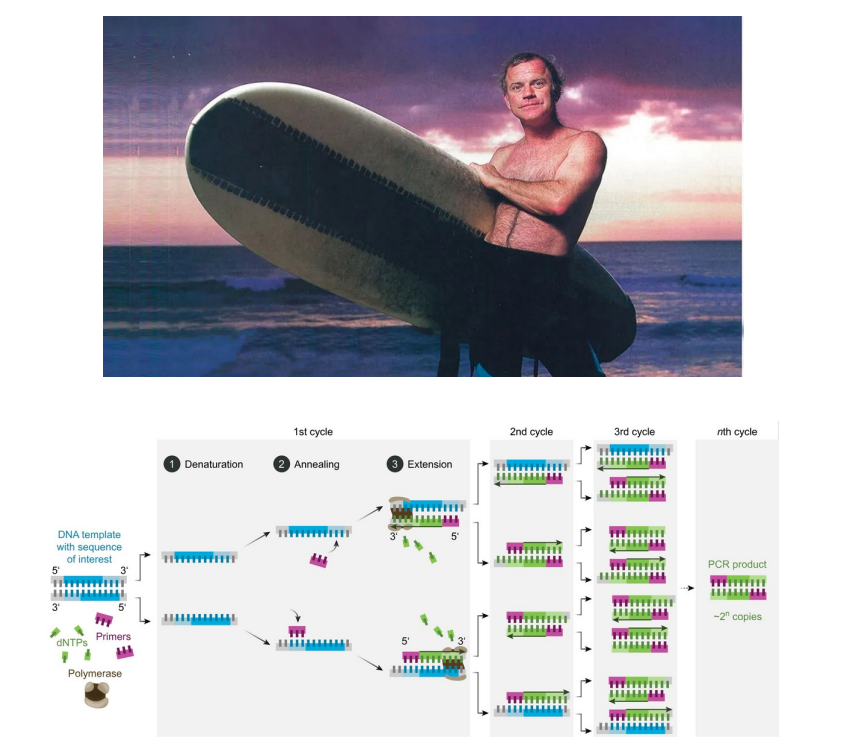
\includegraphics[width=\linewidth]{pcr.png}
        \end{figure}
        \end{column}
    \end{columns}
\end{frame}

\begin{frame}
    \frametitle{Closer Look at PCR}
        \begin{figure}
            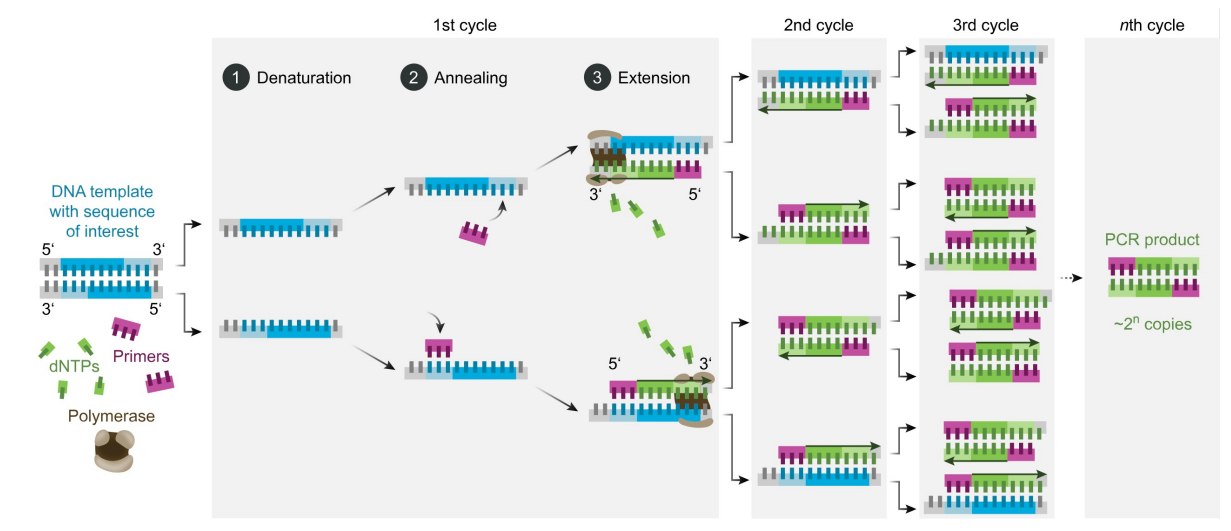
\includegraphics[width=\linewidth]{pcrToo.png}
        \end{figure}
\end{frame}

\begin{frame}
    \frametitle{PCR Specification}
    What is the plan, exactly?

    \begin{itemize}
        \item describe the process in broad, low-resolution terms
        \item check basic properties, discuss {\bf safety} and {\bf liveness}
        \item refine spec by introducing two new variables
        \item refine spec further with {\bf refinement mapping}
        \item check one last property \emph{not expressible} in the first two specs (which are implemented by final spec)
    \end{itemize}
    Let's look at the code!
\end{frame}

\begin{frame}
    \frametitle{But Why?} 
        \begin{itemize}
            \item specs can be refined and checked at each new level of detail
            \item refine it enough and you wind up with pseudocode (PlusCal)
            \item the process of specification improves our understanding of the system
            \item preempt flaws before coding starts
        \end{itemize}
\end{frame}

\end{document} 
